% 2o trabalho de Cálculo 1
% Questões 14 e 26
% Anderson Fraga - Junho 2023

\documentclass[12pt]{article}
\usepackage[a4paper,
            includeheadfoot,
            top=2cm,
            right=2cm,
            bottom=3cm,
            left=3cm]{geometry}
\usepackage[OT1]{fontenc}
\usepackage{parskip, enumitem, pifont, tikz, amssymb, amsmath, hyperref, subcaption}
\usetikzlibrary{calc, shapes}
 % cria os links de referencia das equacoes

\begin{document}

\underline{\textbf{Resolução do Trabalho 2 de Cálculo I}}\par
\textbf{Sistemas de Informação}\\
\textbf{Instituto Federal do Espírito Santo}\\
Campus Serra\par
\textbf{Cálculo I}\\
Prof. Dr. Fábio Lima\par
Anderson A. Fraga (20222BSI0482)\\
\texttt{aafrg@tuta.io}\\  %\texttt formats the text to a typewriter style font

\noindent \underline{\textbf{Cap. 6.4 - Aplicações de integração: Trabalho}}\par
\noindent \textbf{Questão 14 - pág. 407)} Uma corrente é estentdida no chão tem $10 m$ de comprimento e sua massa é $80 kg$. Qual a quantidade de trabalho necessária para levantar uma extremidade da corrente a uma altura de $6 m$?\par
A situação descrita na questão acima pode ser representada como na Figura 1:\par
\begin{figure}[h]
    \centering
    \begin{subfigure}{0.49\textwidth}
        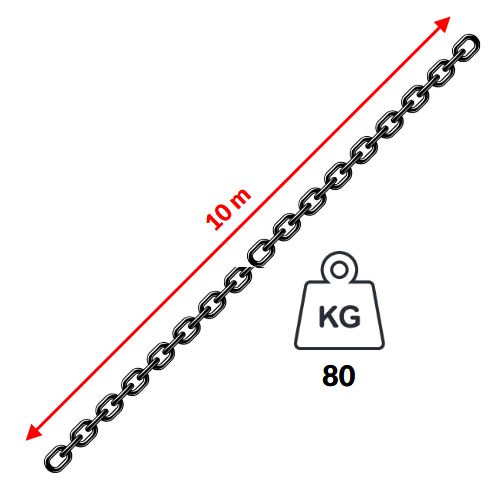
\includegraphics[width=6cm]{fig/fig1.PNG}
    \end{subfigure}
    \begin{subfigure}{0.49\textwidth}
        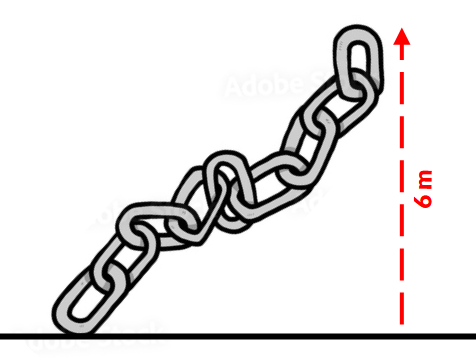
\includegraphics[width=6cm]{fig/fig2.PNG}
    \end{subfigure}
    \caption{\small Comprimento, massa e altura de içamento da corrente.}
\end{figure}\par
Com base na definição 4 tratada no Capítulo 6.4 da referência, onde define que \textbf{trabalho é o movimento feito de um objeto de \emph{a} para \emph{b}}, temos que:\par
\begin{equation}
    \displaystyle W = \lim\limits_{n \to \infty} \sum_{i=1}^{n}f(x_i^*)\Delta x = \int_a^b f(x)dx
\end{equation}
Entretanto, para o caso do levantamento da corrente, podemos reescrever a expressão relacionando inicialmente Força e, consequentemente, as variáveis disponíveis de massa, gravidade e altura de deslocamento da corrente, nas equações seguintes:
\begin{equation}
    \displaystyle W = \int_{a}^{b}Fdx
\end{equation}
E para $F$, Força aplicada para içar a extremidade da corrente de acordo com a altura exigida. Decompondo Força, temos que é o resultado do produto entre a massa, $m$, e a gravidade, $g$, como representado pela equação abaixo:
\begin{equation}
    \displaystyle F = mg
\end{equation}
E, finalmente, podemos determinar que a massa da corrente levantada a uma altura, considerando a densidade da corrente uniforme, pode ser expressa como:
\begin{equation}
    \displaystyle m = \frac{M}{L}x
\end{equation}
Desta forma, substituindo massa na Equação 3 pela Equação 4 e sabendo que deslocaremos a corrente em $6m$, saindo do ponto $a = 0$ até $b = 6$, pode-se utilizar a Equação 2 para determinar o trabalho exigido para levantar uma das extremidades da corrente em $x=6m$, integrando as variáveis constantes e demais incógnitas:\par
\begin{eqnarray}
    \displaystyle W & = &\int_{a}^{b}Fdx \\ \nonumber
    \displaystyle W & = &\int_{0}^{6}\left(\frac{Mg}{L}\right)xdx \\ \nonumber
    \displaystyle W & = &\left(\frac{Mg}{L}\right)\int_{0}^{6}xdx \\ \nonumber
    \displaystyle W & = &\left.\left(\frac{Mg}{L}\right)\left(\frac{x^2}{2}\right)\right|_0^6 \\ \nonumber
    \displaystyle W & = &\frac{80 \times 9,8}{10} \times \frac{36}{2} \\ \nonumber
    \displaystyle W & = & 78.4 \times 18 \\ \nonumber
    \displaystyle W & = & \textrm{1.411,2 J}
\end{eqnarray}
Assim, vemos que o trabalho necessário será de \textbf{1.411,2 joules} para içar uma das extremidades da corrente a 6 metros de altura.\par \vspace{0.25cm}

\noindent \underline{\textbf{Cap. 7.4 - Frações parciais}}\par
\noindent \textbf{Questão 26 - pág. 445)} Escreva as formas de decomposição em frações parciais da função (\textit{como no Exemplo 7}). \textit{Não determine o valor numérico dos coeficientes}.
\begin{equation}
    \int \frac{(x^2+x+1)}{(x^2+1)}dx \tag{1}
\end{equation}
Como descrito na página 438 da referência, o grau do denominador é maior do que o numerador, permitindo, assim, a fatoração do mesmo. Entretanto, o denominador não é um termo fatorável, obrigando a repetição dos termos para o passo seguinte. Junto a fatoração, pode-se, também, expressar a soma das frações parciais resultantes da decomposição da integral inicial. Desta forma, temos:
\begin{equation}
    \frac{(x^2+x+1)}{(x^2+1)}dx \implies \frac{Ax+B}{x^2+1} + \frac{Cx+D}{(x^2+1)^2}  \tag{2}
\end{equation}
Relacionando as frações, temos que:
\begin{equation}
    \frac{(Ax+B)(x^2+1)+Cx+D}{(x^2+1)^2} \nonumber
\end{equation}
Expandindo os termos, chegamos a seguinte expressão:
\begin{equation}
    \frac{Ax^3 + Ax + Bx^2 + B + Cx + D}{(x^2+1)^2} \nonumber
\end{equation}
Rearranjando a expressão, podemos comparar com a integral inicial, onde:
\begin{equation}
    \int \frac{(x^2+x+1)}{(x^2+1)}dx \implies \frac{Ax^3 + Bx^2 + (A+C)x + B + D}{(x^2+1)^2} \tag{3}
\end{equation}
Assim, ao compararmos os termos rearranjados na Equação 3 com os termos do numerador da integral inicial, na Equação 1, percebe-se, a partir desta comparação, que a incógnita A \emph{tem que ser igual a 0} para que a equação do numerador seja válida. Da mesma forma, percebe-se que \emph{B = 1, C = 1 e D necessariamente será igual a 0}.\par
Substituem-se os termos da Equação 2 utilizando os valores encontrados a partir da conclusão da Equação 3, reescrevendo a integral inicial como a soma de duas integrais resultantes da soma de frações parciais. Assim, temos que:
\begin{equation}
    \int \frac{1}{x^2+1}dx + \int \frac{x}{(x^2+1)^2}dx \tag{4}
\end{equation}
Seguindo com a integração da Equação 4, observa-se que a primeira integral tem resultado conhecido, $arcotg x$, enquanto a segunda exige integração por substituição para determinar seu resultado. Desta forma, podemos definir inicialmente que para a segunda integral:
\begin{eqnarray}
    u & = & x^2+1 \\ \nonumber
    du & = & 2xdx \\ \nonumber
    \frac{1}{2}du & = & xdx \\ \nonumber
\end{eqnarray}
\pagebreak

Finalmente, temos que:
\begin{eqnarray}
    & = & \arctan x + \frac{1}{2}\int \frac{1}{u^2}du \\ \nonumber
    & = & \arctan x + \frac{1}{2} \left(-\frac{1}{u}\right)+C \therefore \arctan x - \frac{1}{2(x^2+1)}+C \\ \nonumber
\end{eqnarray}
Complementarmente, podemos visualizar a curva da integral (\emph{Eq. 1}) por meio do gráfico abaixo:
\begin{figure}[h]
    \centering
    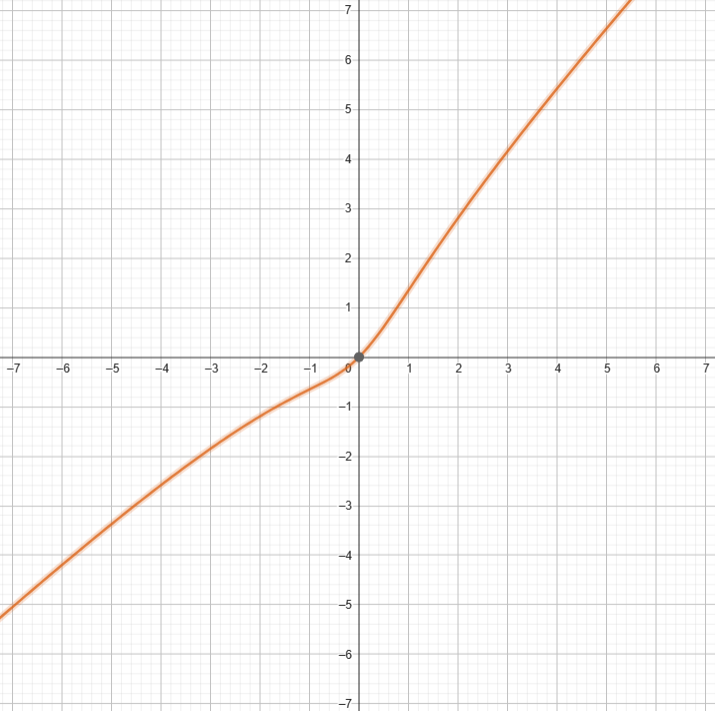
\includegraphics[width=0.8\textwidth]{fig/fig3.PNG}
\end{figure}
\end{document}